\chapter{Building Applications}\label{InputOutput}


\section{Embedding Software}

Embedded programs is in general part of a system comprised of mechanical,
electrical, and/or pneumatic components, and of one or many micro processors 
or even workstations possibly linked by a bus system such as CAN. The embedded
program must interact with these components and it have have access to the
resources of the overall system. In \se, input sensors and output signals 
provide the interface to the environment. Access to the resources is gained 
using native methods.


\subsection{Interfacing to the Environment.}
The interface of a \se\ program to the environment is defined
in terms of \emph{input sensors}\index{sensor!input} and \emph{output signals}\index{signal!output}. We recall the basic facts.

\begin{itemize}
\item A sensor is an input sensor if its constructor has an argument of
type \pp{Input}.

\item A signal is an output signal if its constructor has an argument of
type \pp{Output}.

\item \pp{Input} and \pp{Output} are marker interfaces. 

\item An implementation of the interface \pp{Input}\index{Input@\pp{Input}} requires that
two (callback) methods \pp{new\_val}\index{new\_val@\pp{new\_val}} and \pp{get\_val}\index{get\_val@\pp{get\_val}} are implemented.

For each input sensor, the Boolean method \pp{new\_val} is called at the beginning of an instant. If it returns true, the respective signal is set to 
be present, otherwise it is set to absent. 
Then, if the sensor is valued, the method \pp{get\_val} is called. It must return a value of appropriate type that is the new value of the signal.

\item An implementation of the interface \pp{Output}\index{Output@\pp{Output}} requires that
a method \pp{put\_val}\index{put\_val@\pp{put\_val}}.

For each output signal, the method \pp{put\_val} is called at the 
end of an instant. If the signal is valued it has an argument 
of appropriate type. 
\end{itemize}


\subsection{Native Methods}
Native methods\index{method!native}\index{native} are implemented in a platform-dependent language. 
We use ANSI-C as a host language since cross-compilers are available
for most platforms, in particular if restricted to the small 
subset of ANSI-C as used by the \se\ compiler. 

We have broadened the concept in that not only methods may be native, 
but also constants, and in that \se\ methods may be exported to the
host language. We have the following formats
 
\begin{itemize}
    \item The standard format is
    %
    \BEP
        void native method\_name( \ldots );
    \EEP
    %
    A method \pp{method\_name} is defined by a C function with the same name.


    \item The native method may be renamed
    %
    \BEP
        void native("method\_name") se\_method\_name( \ldots );
    \EEP
    %    
    The method \pp{se\_method\_name} is defined by the C function
    \pp{method\_name}

    \item  Methods defined in \se\ may be exported
    %
    \BEP
        void export\_to\_C method\_name( \ldots ) \{
            \ldots
        \};
    \EEP
    %
    The function \pp{method\_name} may be called in C to execute
    the method.
    
    
    \item The exported method may be renamed

    %
    \BEP
        void export\_to\_C(method\_name) se\_method\_name( \ldots ) \{
        \ldots
        \};
        \EEP
    %    
    The function \pp{method\_name} may be called in C to execute the
    method \pp{se\_method\_name} 


    \item  Constants, i.e. fields that are static and final, may be 
    imported from C or exported to C using the same modifiers as used 
    for methods. 
\end{itemize}

Whether methods or constants are imported or exported is often a
matter of taste.  However, if such constants or methods are often
changed it is probably more convenient to export since development
takes place in the same framework.  In contrast, it might be useful
 to import in order to hide details of 
implementation. 

Import and export of constants is useful in particular since \java\
lacks enumerations.  since enumerations are typically defined by a
list of constants the \se\ program and C environment should agree
about such enumeriations which is best achieved if the enumerations 
are only defined once and then imported or exported.

\section{Interfacing to the Environment}

The following example demonstrates how interfaces may be implemented using
native methods. The example can be found in\\ 
\pp{\$SE\_HOME$\backslash$target$\backslash$examples$\backslash$Blink4}.

\paragraph{Reactive behaviour.}
The reactive behaviour of the program is specified by the reactive method
%
\codefragment{blink4-rct}
%
There is an hierarchic automaton with two states \pp{select\_green} and \pp{select\_red}. The automaton changes state if the sensor \pp{select}
is present. Each of the states host an automaton. Each of these automata
toggles between emittance and non-emittance of an output signal, \pp{red\_on}
for the state \pp{select\_red}, and \pp{red\_green} for the state \pp{select\_green}. The toggle is applied if the input sensor \pp{toggle} is
present.

\paragraph{Interfaces of sensors and signals.} 
We use a very simple idea for interfacing: each of input sensors and
output signals is known in the environment by its name as a
string. This name is passed on to the environment, either for checking for
presence with \pp{new\_val}, or when calling \pp{put\_val}.

Here is the implementation for inputs
%
\codefragment{blink4-input-button}
%
Calling the constructor stores the ``button name''. The parameterless method 
\pp{new\_val} just calls a method \pp{new\_val} with the button name being
parameter. The latter method is native, the implementing function being 
\pp{getPresence}.

An object of class \pp{InputButton} is then used to initialise the signal
\pp{toggle} in
%
\codefragment{blink4-toggle}
%
Alternatively, one might have declared an object of type \pp{InputButton}
that is used in a sensor constructor as in
%
\codefragment{blink4-select}
%

For output signals, we implement the interface \pp{Output} similarly
%
\codefragment{blink4-output-led}
%
The method \pp{put\_val} essentially calls the function \pp{printStdout}
of the environment.

A variation of the theme is define the method \pp{stdOutput} on class level
and to use an anonymous class
%
\codefragment{blink4-red-on}
%
\paragraph{The method \pp{main}.}
The method \pp{main} consists of a while loop.
%
\codefragment{blink4-main}
%
The condition of the while loop is a conjunction of two conditions.
The first condition consists of the method call \pp{read\_input}.
The method is native. It ``reads'' the input sensors as we will
see when analysing the corresponding C-code below. It is called at the beginning of an instant since it is executed before the second condition is evaluated. The second condition is the familiar call of the method \pp{instant}. 

\paragraph{The native code.}

The native code specifies all the native functions.   
\BEP
\#include <stdio.h>
\#include <string.h>
\#include <ctype.h>
\#include <stdlib.h>
\#include "se.Blink4.h" /* as generated by the sE-compiler */
\EEP

For checking the presence of input sensors we have the following code

\BEP
Bool selectPresence, togglePresence;

Bool getPresence (char *s) \{
  if (strcmp(s,"select") == 0) \{
     return selectPresence;
  \} else if (strcmp(s,"toggle") == 0) \{
     return togglePresence;
  \} else \{
     fprintf (stdout,"invalid getPresence returned FALSE$\backslash$n");
     fflush (stdout);
     return FALSE;
  \};
\}
\EEP
For each input sensor, a Boolean variable is declared. The variables
encode the status; if a variable is true, the sensor is present, otherwise
it is absent.
The function \pp{getPresence} checks whether a sensor is present or not.
Its arguments is a string that is matched with the names of the input
sensors. If the argument matches a signal name its status is returned.
If no signal name matches an error message is written to \pp{stdout}.

\BEP
Bool readInput (void) \{
  selectPresence = FALSE;
  togglePresence = FALSE;
  while ( fgets(zLine,20,stdin) ) \{
    if (zLine[0] == 'q') \{
       fprintf (stdout,"exit (0)$\backslash$n");
       fflush (stdout);
       return FALSE;
    \} else if (zLine[0] == 't') \{
       togglePresence = TRUE;
    \} else if (zLine[0] == 's') \{
       selectPresence = TRUE;
    \} else if (zLine[0] == '.') \{
       return TRUE;
    \} else \{
        fprintf (stdout,"input ignored$\backslash$n");
        fflush (stdout);
    \};
  \};
  return FALSE;
\}
\EEP

\section{Interfacing with the Environment - continued}



\section{Building a Project}

The \se\ environment supports a very elementary project handling. A \emph{project}
consists of a directory that includes all the files relevant to a particular 
application such as \se\ files, \se charts files, C files, and C libs, and a particular
\emph{project resource file} \pp{.seprj} which is generated by using 
the \emph{project panel} but which may be edited by hand. 
\begin{figure}[h]
\begin{center}
    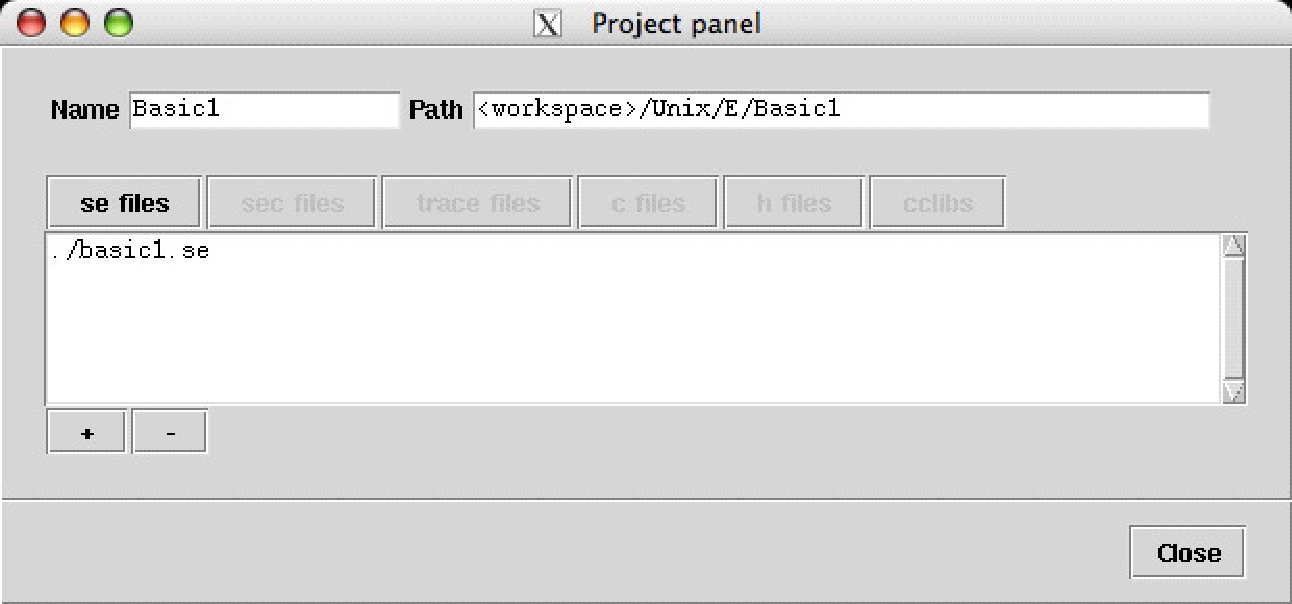
\includegraphics[width=250pt]{../pdf/synerjy-project}
\end{center}
\caption{The synERGY project panel}
\end{figure}\label{project-panel}
Here we consider the project \pp{\$SE\_HOME$\backslash$target$\backslash$examples$\backslash$Blink4} which consists of the files discussed above.

Building of an application is discussed in the \se\ user manual but a few
additional remarks may be useful. For maximal flexibility we use makefiles
for building and running an application. The \pp{Build}
button at first generates a file \pp{Makefile.gen} in \pp{\$SE\_HOME/tmp}
%
\BEP
SE\_MAKEINFO=makeinfo
SE\_WORKSPACE=/Users/ap/Unix/E/Blink4
SE\_BINARY=se.a.out
SE\_CPROGRAM=/Users/ap/Unix/E/Blink4/se.Blink4.c
SE\_CFILES=/Users/ap/Unix/E/Blink4/blink4.c 
SE\_CLIBS=
\EEP
%
in case of the example.

This file is included in a generic \pp{Makefile} in the directory
 \pp{\$SE\_HOME/target/\emph{host}}. The structure of the generic \emph{Makefile}
is as follows
%
\BEP
-include \$(SE\_HOME)/tmp/Makefile.gen

sim: 
        gcc \$(SE\_CPROGRAM) \$(SE\_CFILES) -o \$(SE\_BINARY) $\backslash$
            -Dse\_sim $\backslash$
            -Dse\_\_linux $\backslash$
            -I \$(SE\_HOME)/include $\backslash$
            -I include $\backslash$
            -I \$(SE\_HOME)/target/linux/include $\backslash$
	        \$(SE\_HOME)/target/linux/lib/libse\_rt.a $\backslash$
	        -lm -lpthread

tgt:
        gcc \$(SE\_CPROGRAM)  \$(SE\_CFILES) -o \$(SE\_BINARY) $\backslash$
	        -Dse\_\_linux $\backslash$
	        -I \$(SE\_HOME)/include  $\backslash$
	        -I \$(SE\_HOME)/target/linux/include $\backslash$
	        \$(SE\_HOME)/target/linux/lib/libse\_rt.a $\backslash$
	        -lm -lpthread

sfun:
        mex \$(SE\_CPROGRAM)  \$(SE\_CFILES) -output \$(SE\_BINARY) $\backslash$
            -Dse\_\_linux $\backslash$
            -I\$(SE\_HOME)/include $\backslash$
            -I\$(SE\_HOME)/target/linux/include $\backslash$
            \$(SE\_HOME)/target/linux/lib/libse\_rt.a

run:
        exec xterm -e \$(SE\_BINARY)

clean:
        rm -f \$(SE\_PREFIX)*
\EEP
%
There are several rules according to target.
\begin{itemize}
\item[\pp{sim}] A rule to invoke the simulator.

\item[\pp{tgt}] A rule to generate code for the host machine.

\item[\pp{sfun}] A rule to generate an Sfunction for import to Simulink.

\item[\pp{run}] A rule to run the application. Here it is executed in a terminal.
For microprocessors, this typically implies upload.

\end{itemize}

The Makefiles may be replaced according to one's taste but be careful to use the
same rules names if the \se\ environment is to be used. The better alternative
is to include a self-defined Makefile in the project directory. This will
then be called automatically instead of the predefined ones.


\section{Using Makefiles only.}

The final alternative for the friends of the hard-core approach is to use
Makefiles exclusively forgetting about soft programming environments: there
is a reasobly exprissive command language to deal with most problems on the
level of command lines or - for comfort - in a Makefile. Here is an example

\BEP
include \$SE\_HOME/target/unix/include/Makefile.inc

\# example blink4.se needs external C
now: se.Blink4

se.Blink4.c: blink4.se
	se -f "%load file=blink4.se; $\backslash$
               set target=linux;set hfile=se\_rt.h; $\backslash$
               make C-code;quit;"

se.Blink4: se.Blink4.o blink4.o
	\$(CC) -o se.Blink4 se.Blink4.o blink4.o $\backslash$
              \$(SE\_HOME)/target/unix/lib/libsert.a

\# misc stuff ******************************************************
doc: clean
	doxygen

clean:
	rm -f se.* *.o
	rm -rf html rtf man latex
	rm -rf se.*
	rm -rf sim/se.*
	rm -rf target/se.*
\EEP
The \pp{Makefile.incl} sets several variables in a uniform way. The general strategy of writing Makefiles is to  use one rule to execute two steps
\begin{itemize}
\item
generate the \pp{se.<ConfigurationClass>.c} file from the synERJY-sources
(as it is done in the \pp{se.Blink4.c} - rule)

\item
compile and link the application (as it is done in the \pp{se.Blink4} rule)

\end{itemize}

%\section{An Interface for LEGO Mindstorms}

%To be written
%% ?????????

%\section{A Microprocessor Example}

%To be written
%% ?????????

%\section{A CAN bus example}

%To be written
%% ?????????







